\documentclass{homework}

\usepackage{pdfpages, float}
\usepackage{wrapfig, graphicx}
\usepackage{enumitem, subcaption}
\usepackage{lmodern}
\usepackage[strings]{underscore}
\def\mathdefault#1{#1}

% pacotes para importar código
\usepackage{caption, booktabs, fancyvrb, makecell}
\usepackage[inkscapepath=build/inkscape]{svg}
\usepackage[section, newfloat]{minted}

\definecolor{monokaibg}{HTML}{272822}
\definecolor{monokaitext}{HTML}{F8F8F2}

% https://github.com/gpoore/minted/issues/84
\renewcommand{\FancyVerbFormatLine}[1]{\textcolor{monokaitext}{~#1}}

\setminted{
    bgcolor = monokaibg,
    style   = monokai,
    frame   = leftline,
    framesep = 2mm,
    autogobble,
    samepage,
    python3,
    breaklines,
    escapeinside=!!,
}

\setmintedinline{
    autogobble=false,
}

\usepackage{csquotes}
\usepackage[section]{placeins}

\usepackage[hidelinks]{hyperref}
\usepackage[noabbrev, nameinlink, brazilian]{cleveref}
\hypersetup{
    pdftitle  = {MC833 - Projeto 3 - RA187679},
    pdfauthor = {Tiago de Paula}
}

% \captionsetup[listing]{position=below,skip=-1pt}
\SetupFloatingEnvironment{listing}{name=Trecho de Código}
\crefname{listing}{código}{códigos}
\Crefname{listing}{Código}{Códigos}

\crefname{appendix}{apêndice}{apêndices}
\Crefname{appendix}{Apêndice}{Apêndices}

\usepackage[most]{tcolorbox}

\newtcolorbox{ghostbox}[1][]{
    blank,
    breakable,
    left = 0pt,
    right = 0pt,
    top = 0pt,
    bottom = 0pt,
    #1
}

\usepackage{titlesec}

\makeatletter
\g@addto@macro\appendix{
    \titleformat{\section}
    {\normalfont\Large\bfseries}
    {\appendixname~\thesection:}
    {1em}{}

    \crefalias{section}{appendix}
}
\makeatother

\usepackage{import, multirow}
\usepackage{pgf, tikz}
\usetikzlibrary{matrix}
\usetikzlibrary{positioning}
\usetikzlibrary{automata}
\usetikzlibrary{shapes}

\usepackage{multicol}
\usepackage{physics}

\usepackage[per-mode = symbol]{siunitx}
% recreate \qty
\AtBeginDocument{\RenewCommandCopy\qty\SI}
% ignore \qty warnings
\ExplSyntaxOn
\msg_redirect_name:nnn{siunitx}{physics-pkg}{none}
\ExplSyntaxOff

% bits and bytes per second
\DeclareSIUnit{\bps}{\bit\per\second}
\DeclareSIUnit{\Bps}{\byte\per\second}

\usepackage{silence}

\WarningFilter*{latex}{Text page \thepage\space contains only floats}

\title{
    \vspace{-2\baselineskip}
    Projeto 3: \\
    {\Large Previsão de tráfego de rede com Redes Neurais Recorrentes}
}

\author{
    Tiago de Paula Alves ~(187679) \\
    \href{mailto:t187679@dac.unicamp.br}{\texttt{t187679@dac.unicamp.br}}%
}

\begin{document}
\maketitle\thispagestyle{fancy}
\vspace{-3em}

\pagestyle{main}

\section{Introdução}

Este projeto tem como objetivo modelar o tráfego em uma rede de computadores utilizando redes neurais
recorrentes (LSTM). Para isso, utilizamos um arquivo de captura de pacotes (PCAP) da base pública MAWI/CAIDA,
construímos uma série temporal de bytes por segundo e, por fim, treinamos um modelo LSTM para prever o
próximo valor da série.
A metodologia adotada e os resultados obtidos são detalhados nas seções subsequentes.

\section{Análise Exploratória de Dados (EDA)}

A primeira etapa do projeto consistiu em realizar uma análise exploratória sobre os dados de tráfego para
compreender suas características fundamentais.
O \emph{dataset} original, após ser processado, resultou em uma série temporal de volume de tráfego agregado
por segundo.

\begin{table}[!htb]
    \centering
    \caption{Estatísticas descritivas para a série temporal de \texttt{bytes\_per\_second}.}
    \label{tab:eda-describe}
    ../../results/200701251400.describe.tex
\end{table}

A \Cref{tab:eda-describe} apresenta as estatísticas descritivas da série.
[... Adicione seus comentários aqui sobre a média, desvio padrão, e a faixa de valores (min/max) ...]

\begin{figure}[!htb]
    \centering
    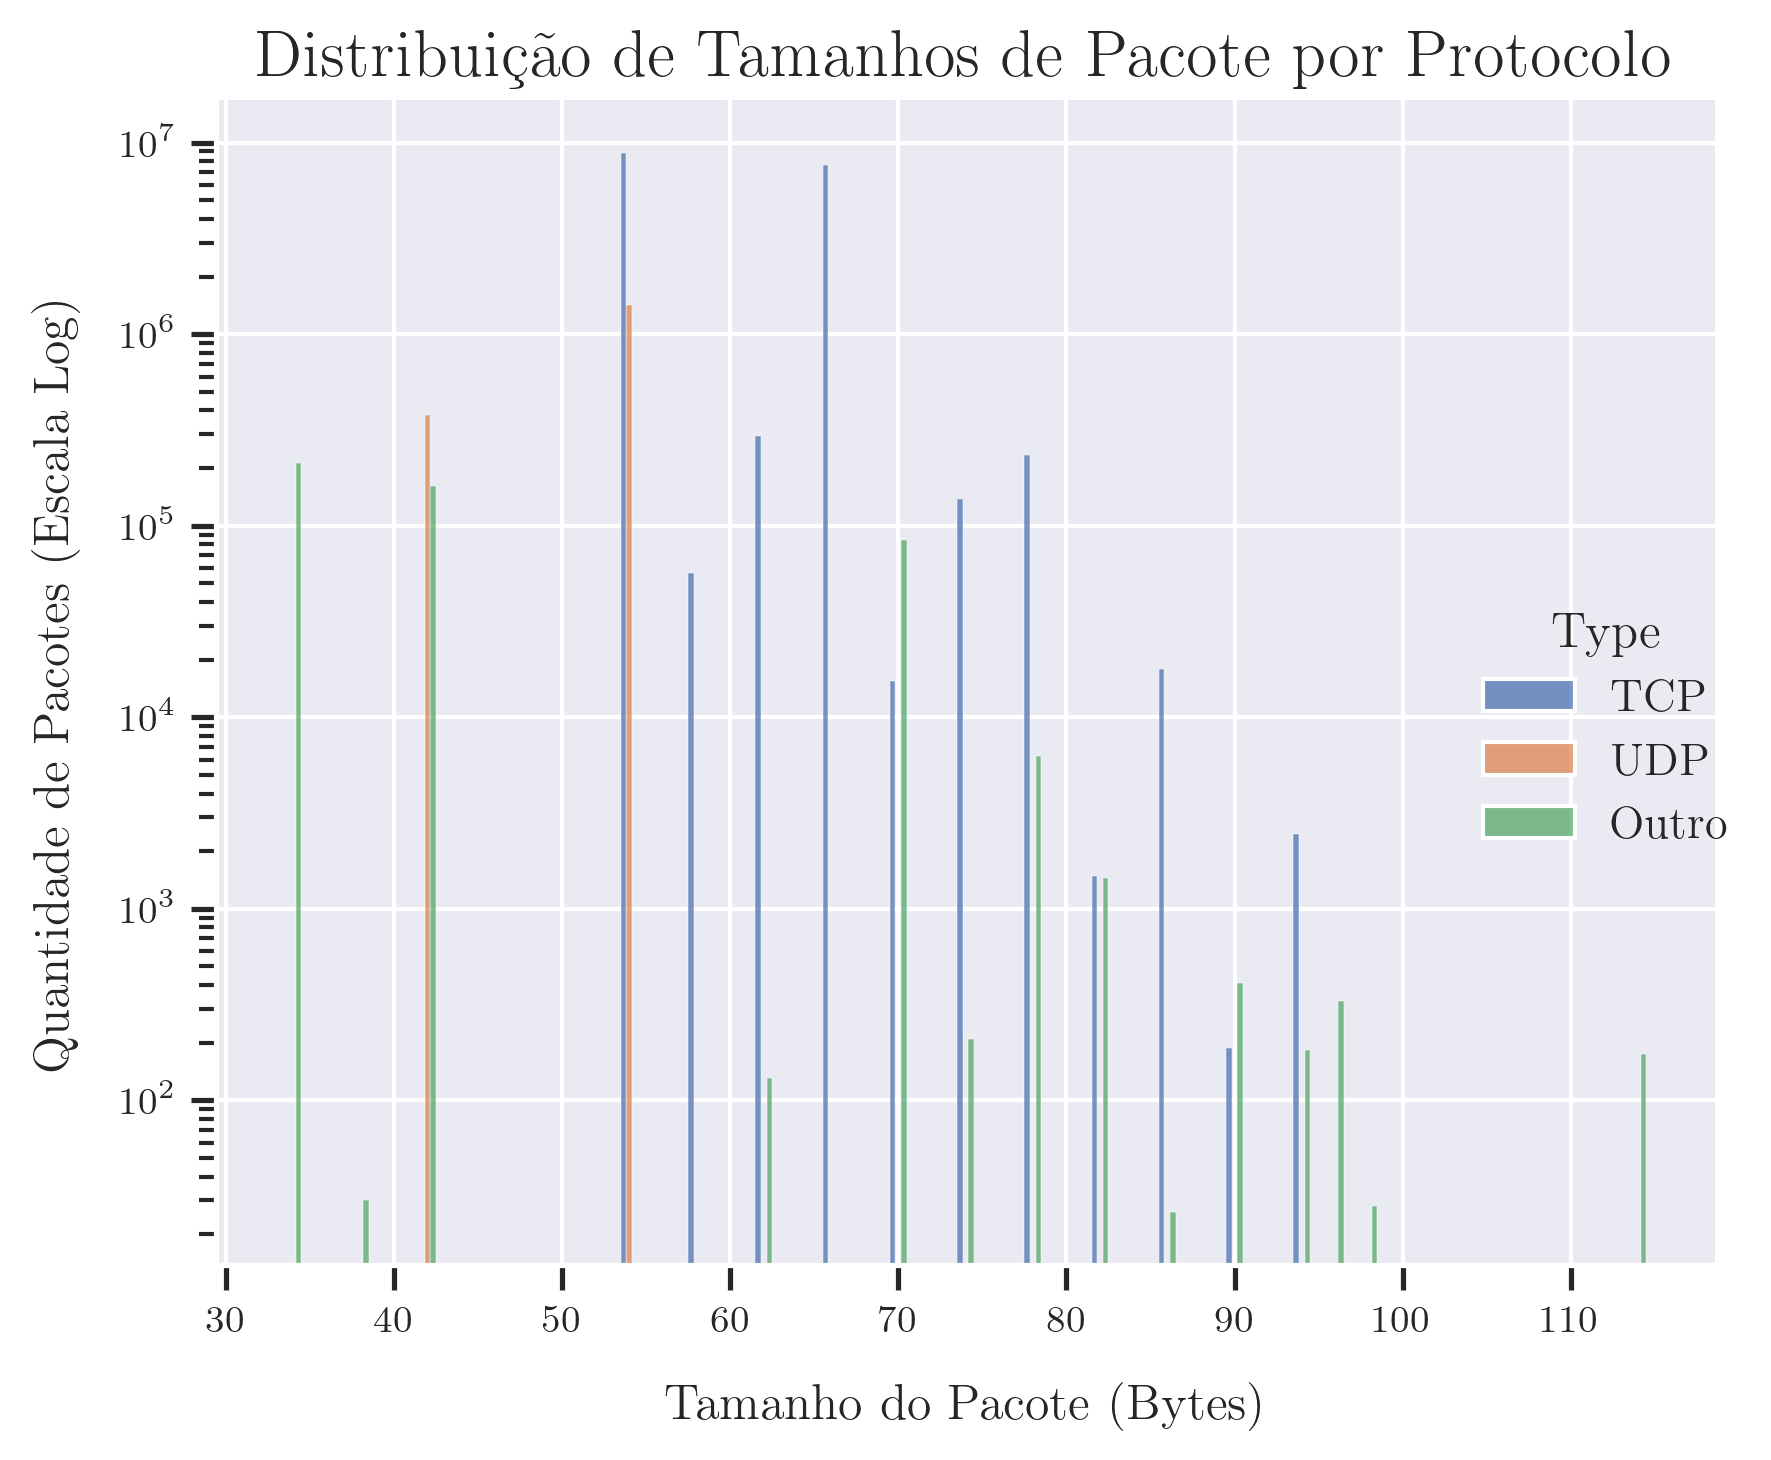
\includegraphics[width=0.95\textwidth]{resource/200701251400.protocol_dist.png}
    \caption{Distribuição de tamanhos de pacote para os protocolos TCP e UDP. A frequência (eixo Y) está em
    escala logarítmica para melhor visualização.}
    \label{fig:eda-protocol-dist}
\end{figure}

A \Cref{fig:eda-protocol-dist} ilustra a distribuição dos tamanhos de pacote.
[... Adicione seus comentários aqui, observando por exemplo os picos de pacotes pequenos (ACKs TCP) e grandes
(dados) ...]

\begin{figure}[!htb]
    \centering
    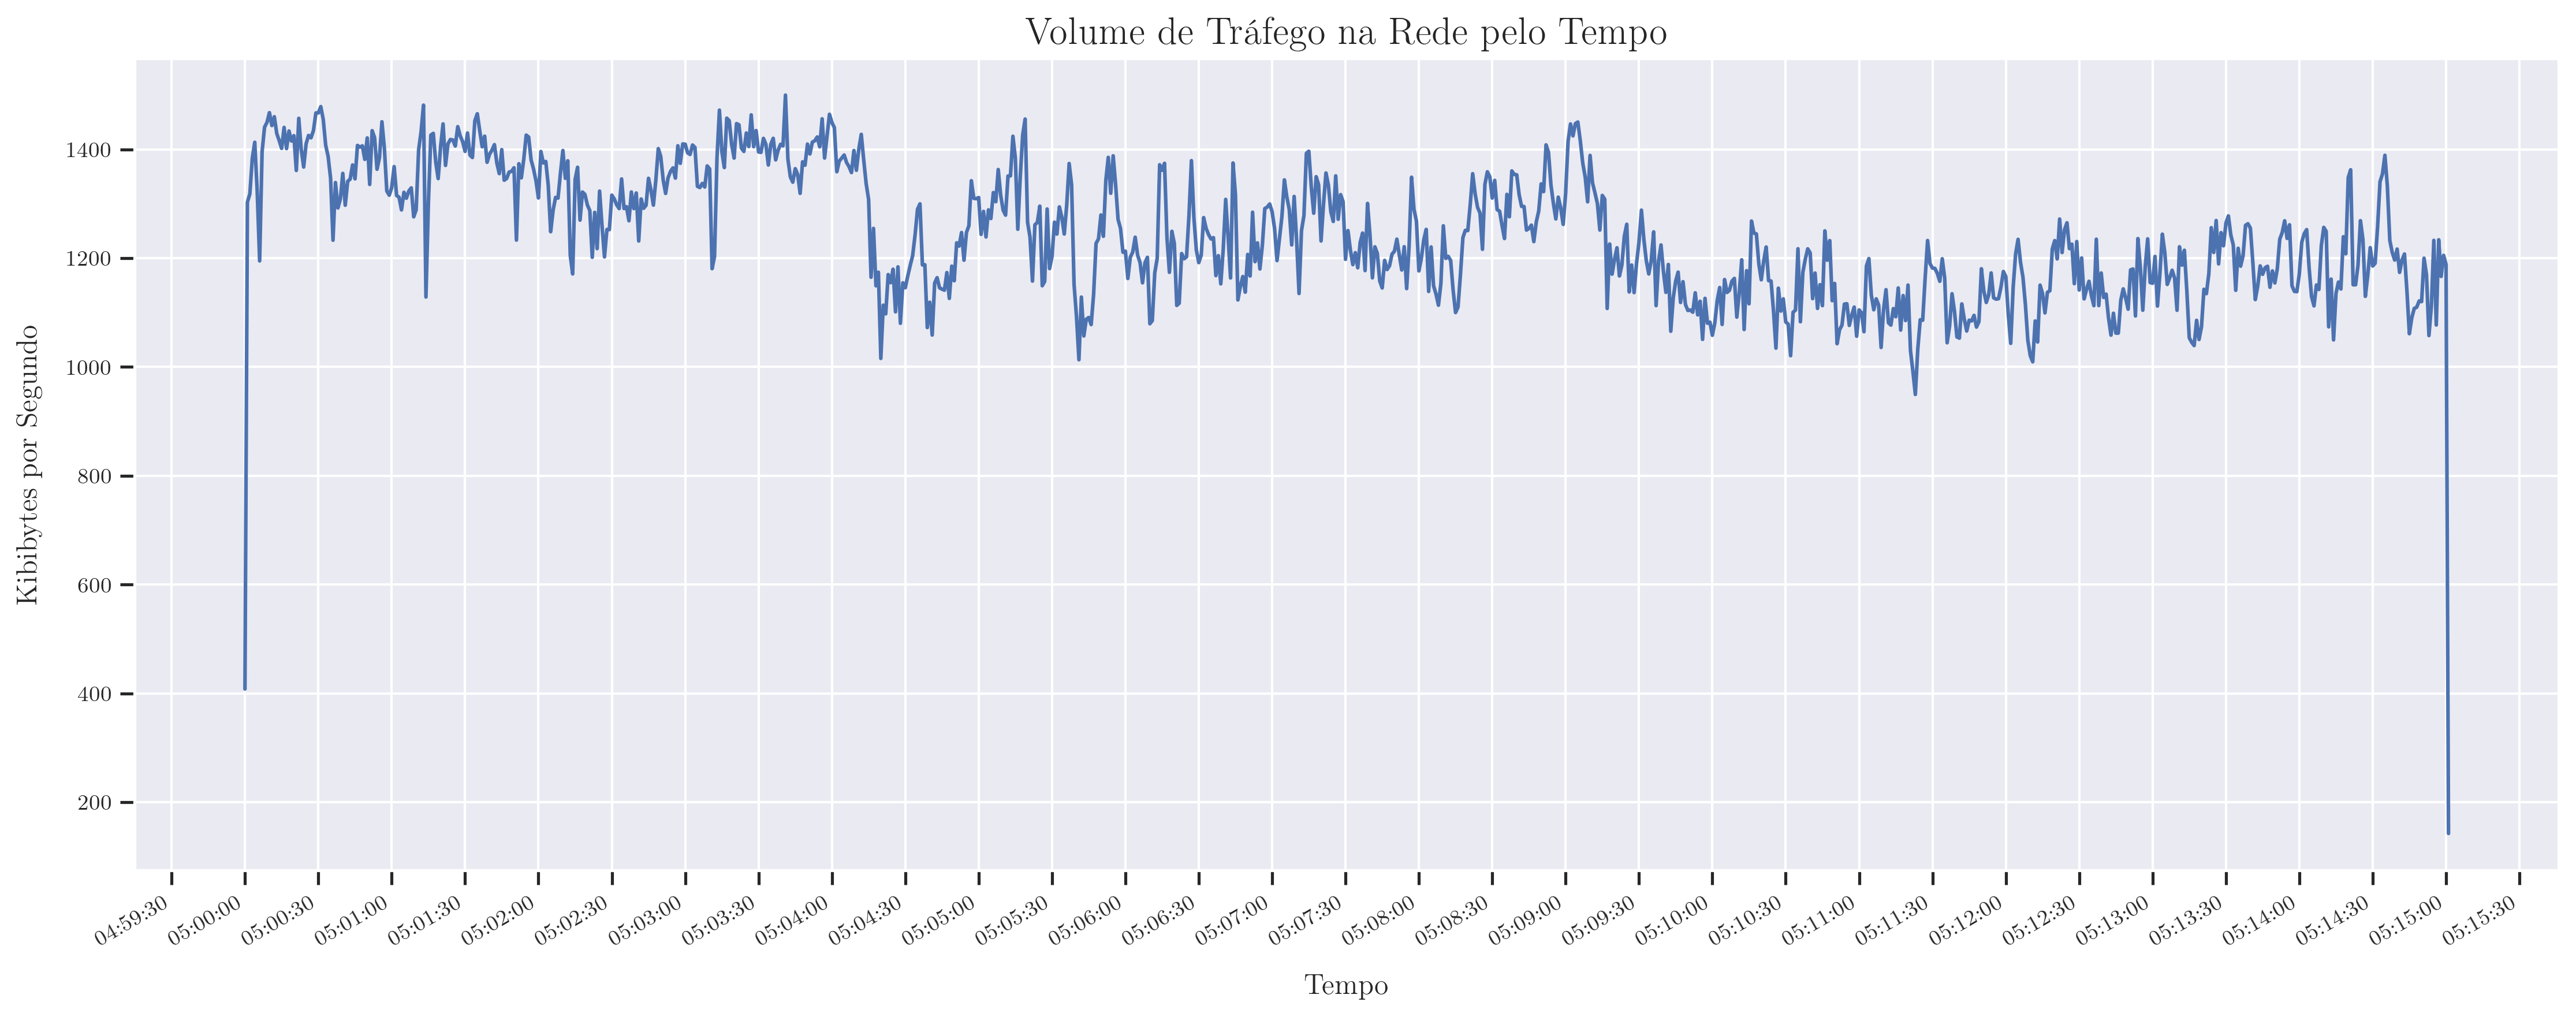
\includegraphics[width=0.95\textwidth]{resource/200701251400.time_series.png}
    \caption{Série temporal do volume de tráfego agregado por segundo.}
    \label{fig:eda-timeseries}
\end{figure}

A \Cref{fig:eda-timeseries} mostra o comportamento do tráfego ao longo do tempo.
[... Adicione seus comentários sobre a volatilidade, picos e períodos de estabilidade ...]

\begin{figure}[!htb]
    \centering
    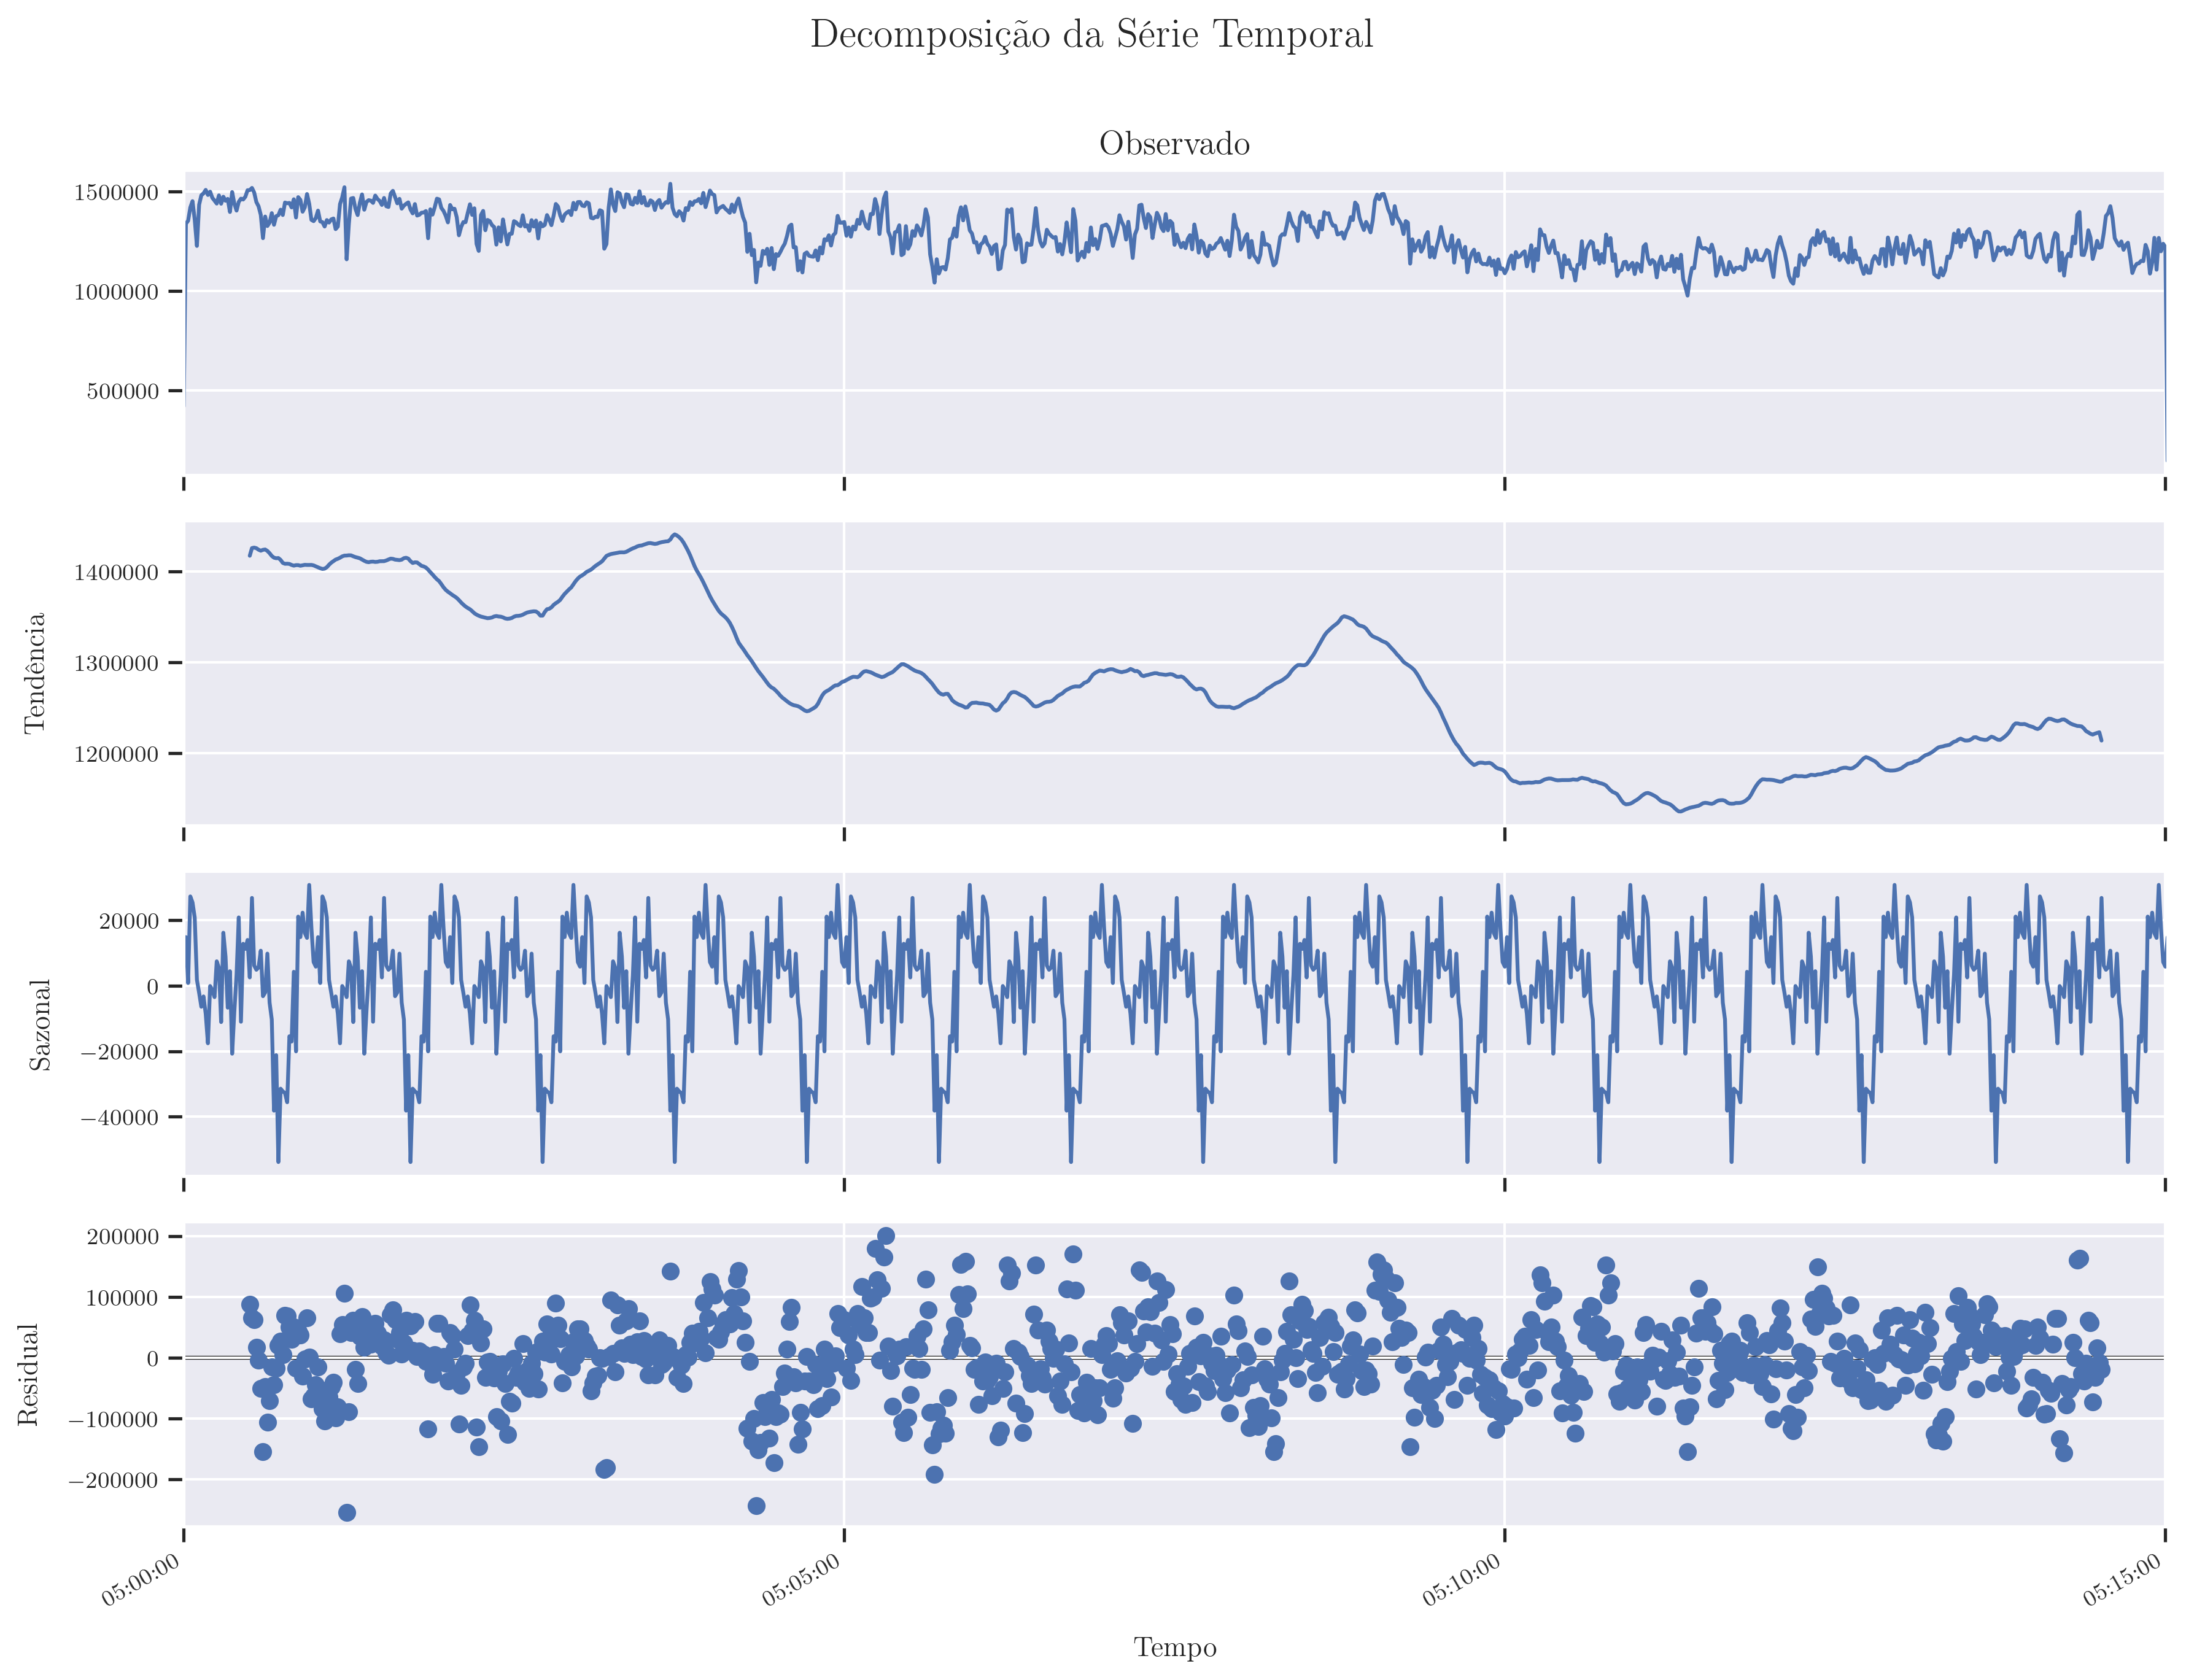
\includegraphics[width=0.8\textwidth]{resource/200701251400.decomposition.png}
    \caption{Decomposição da série temporal em tendência, sazonalidade e resíduos, com um período sazonal de
    60 segundos.}
    \label{fig:eda-decomposition}
\end{figure}

Para uma análise mais aprofundada, decompomos a série em seus componentes de tendência, sazonalidade e
resíduos, como visto na \Cref{fig:eda-decomposition}.
[... Adicione seus comentários sobre a tendência de longo prazo e os padrões periódicos (sazonais) que o
modelo precisará aprender ...]

\begin{figure}[!htb]
    \centering
    \includegraphics[width=0.7\textwidth]{resource/200701251400.autocorrelation.png}
    \caption{Funções de Autocorrelação (ACF) e Autocorrelação Parcial (PACF) para a série temporal.}
    \label{fig:eda-acf-pacf}
\end{figure}

Finalmente, a \Cref{fig:eda-acf-pacf} mostra as funções de autocorrelação. O decaimento lento da ACF confirma
a presença de uma forte tendência. A PACF, por sua vez, mostra correlações significativas nos primeiros lags,
justificando o uso de uma janela de look-back para o modelo LSTM.
[... Adicione seus comentários ...]

\section{Modelamento Preditivo}

Para a previsão do tráfego, foi implementado um modelo de Redes Neurais Recorrentes do tipo LSTM (\emph{Long
Short-Term Memory}), conforme especificado. A arquitetura adotada foi enxuta, consistindo em uma camada LSTM
com 50 unidades, seguida por uma camada Densa com uma única saída para prever o valor do próximo segundo. A
preparação dos dados envolveu a normalização da série de \texttt{bytes\_per\_second} para o intervalo [0, 1]
e a criação de sequências de entrada utilizando uma janela deslizante (\emph{look-back}).

\subsection{Resultados com o Dataset Curto (15 minutos)}

Inicialmente, foram conduzidos experimentos com o \emph{dataset} \texttt{200701251400.dump.gz}, que abrange
um período de 15 minutos de captura. Foram testados quatro tamanhos de janela distintos: 10, 20, 30 e 60
segundos, com 50 épocas de treinamento e um \emph{batch size} de 64. A performance de cada modelo foi
avaliada no conjunto de teste utilizando a métrica de Erro Quadrático Médio (MSE).

\begin{table}[!htb]
    \centering
    \caption{Resultados de MSE para diferentes configurações de \emph{look-back} com o \emph{dataset} de 15
    minutos. O modelo com \texttt{look\_back=20} apresentou a melhor performance.}
    \label{tab:modeling-mse-short}
    \begin{tabular}{cc}
    \toprule
    Look Back & MSE \\
    \midrule
    10 & 11242733286.49 \\
    20 & 10432004668.86 \\
    30 & 11655084093.13 \\
    60 & 11419691841.78 \\
    \bottomrule
\end{tabular}

\end{table}

Os resultados na \Cref{tab:modeling-mse-short} indicam que a janela de \texttt{look\_back=20} segundos obteve
o menor MSE. Isso sugere que, para esta série temporal curta e relativamente estável, um histórico de 20
segundos forneceu o melhor equilíbrio entre contexto e ruído para a previsão.

A \Cref{fig:modeling-prediction-short} compara visualmente a previsão do melhor modelo com os dados reais. O
modelo consegue capturar a tendência geral e a sazonalidade de baixa frequência do tráfego. No entanto, as
previsões são notavelmente mais suaves que os dados reais, evidenciando uma dificuldade em modelar os picos
de alta frequência, o que é um comportamento esperado para uma arquitetura simples em uma série com ruído.

\begin{figure}[!htb]
    \centering
    \includegraphics[width=0.95\textwidth]{resource/200701251400.prediction.e50.b64.png}
    \caption{Comparação entre os valores reais e previstos pelo melhor modelo (\texttt{look\_back=20}) no
    \emph{dataset} de 15 minutos. O modelo segue a tendência, mas suaviza as flutuações de alta frequência.}
    \label{fig:modeling-prediction-short}
\end{figure}

\FloatBarrier
\subsection{Resultados com o Dataset Longo (9 horas)}

Para avaliar o modelo em um cenário mais realista com padrões de longo prazo, os mesmos experimentos foram
replicados no \emph{dataset} \texttt{200701011800.dump.gz}, que abrange quase 9 horas.

\begin{table}[!htb]
    \centering
    \caption{Resultados de MSE para o \emph{dataset} de 9 horas. Novamente, a janela de
    \texttt{look\_back=20} se mostrou a mais eficaz.}
    \label{tab:modeling-mse-long}
    \begin{table}
    \caption{Mean Squared Error for Different Look-Back Windows}
    \label{tab:mse_results}
    \begin{tabular}{lrr}
        \toprule
        & Look Back & MSE \\
        \midrule
        0 & 10 & 6032583.47 \\
        1 & 20 & 6050556.08 \\
        2 & 30 & 5994997.67 \\
        \bottomrule
    \end{tabular}
\end{table}

\end{table}

Como mostra a \Cref{tab:modeling-mse-long}, a janela de \texttt{look\_back=20} novamente apresentou o melhor
desempenho. Mais notavelmente, os valores de MSE são ordens de magnitude menores em comparação com o dataset
curto. Isso ocorre porque o tráfego no dataset longo possui uma linha de base muito mais baixa e estável, com
picos de tráfego sendo eventos mais raros, embora de altíssima magnitude.

\begin{figure}[!htb]
    \centering
    \includegraphics[width=0.95\textwidth]{resource/200701011800.prediction.e50.b64.png}
    \caption{Comparação entre os valores reais e previstos pelo melhor modelo (\texttt{look\_back=20}) no
        \emph{dataset} de 9 horas. O modelo prevê a linha de base com alta precisão, mas falha completamente em
    antecipar os picos de tráfego.}
    \label{fig:modeling-prediction-long}
\end{figure}

A \Cref{fig:modeling-prediction-long} revela a principal característica do modelo neste cenário: ele se torna
um excelente preditor da linha de base do tráfego. O modelo aprende a ignorar a variância extrema e prevê com
precisão o comportamento do tráfego durante os longos períodos de baixa atividade. No entanto, ele falha
completamente em prever os picos súbitos e massivos de tráfego. O modelo não aprendeu a antecipar esses
eventos de "cisne negro", tratando-os como ruído imprevisível e mantendo sua previsão próxima da média histórica.

\subsection{Resultados com Tamanho de Batch Reduzido}
Adicionalmente, foi realizado um experimento no \emph{dataset} curto com hiperparâmetros reduzidos (20 épocas
e \emph{batch size} de 32) para avaliar a sensibilidade do modelo.

\begin{table}[!htb]
    \centering
    \caption{Resultados de MSE para o \emph{dataset} \texttt{200701251400.dump.gz} com 20 épocas e
    \emph{batch size} de 32.}
    \label{tab:modeling-mse-reduced}
    \begin{tabular}{cc}
    \toprule
    Look Back & MSE \\
    \midrule
    10 & 11814694510.86 \\
    20 & 10691583376.90 \\
    30 & 11310507183.37 \\
    60 & 13703889350.77 \\
    \bottomrule
\end{tabular}

\end{table}

\begin{figure}[!htb]
    \centering
    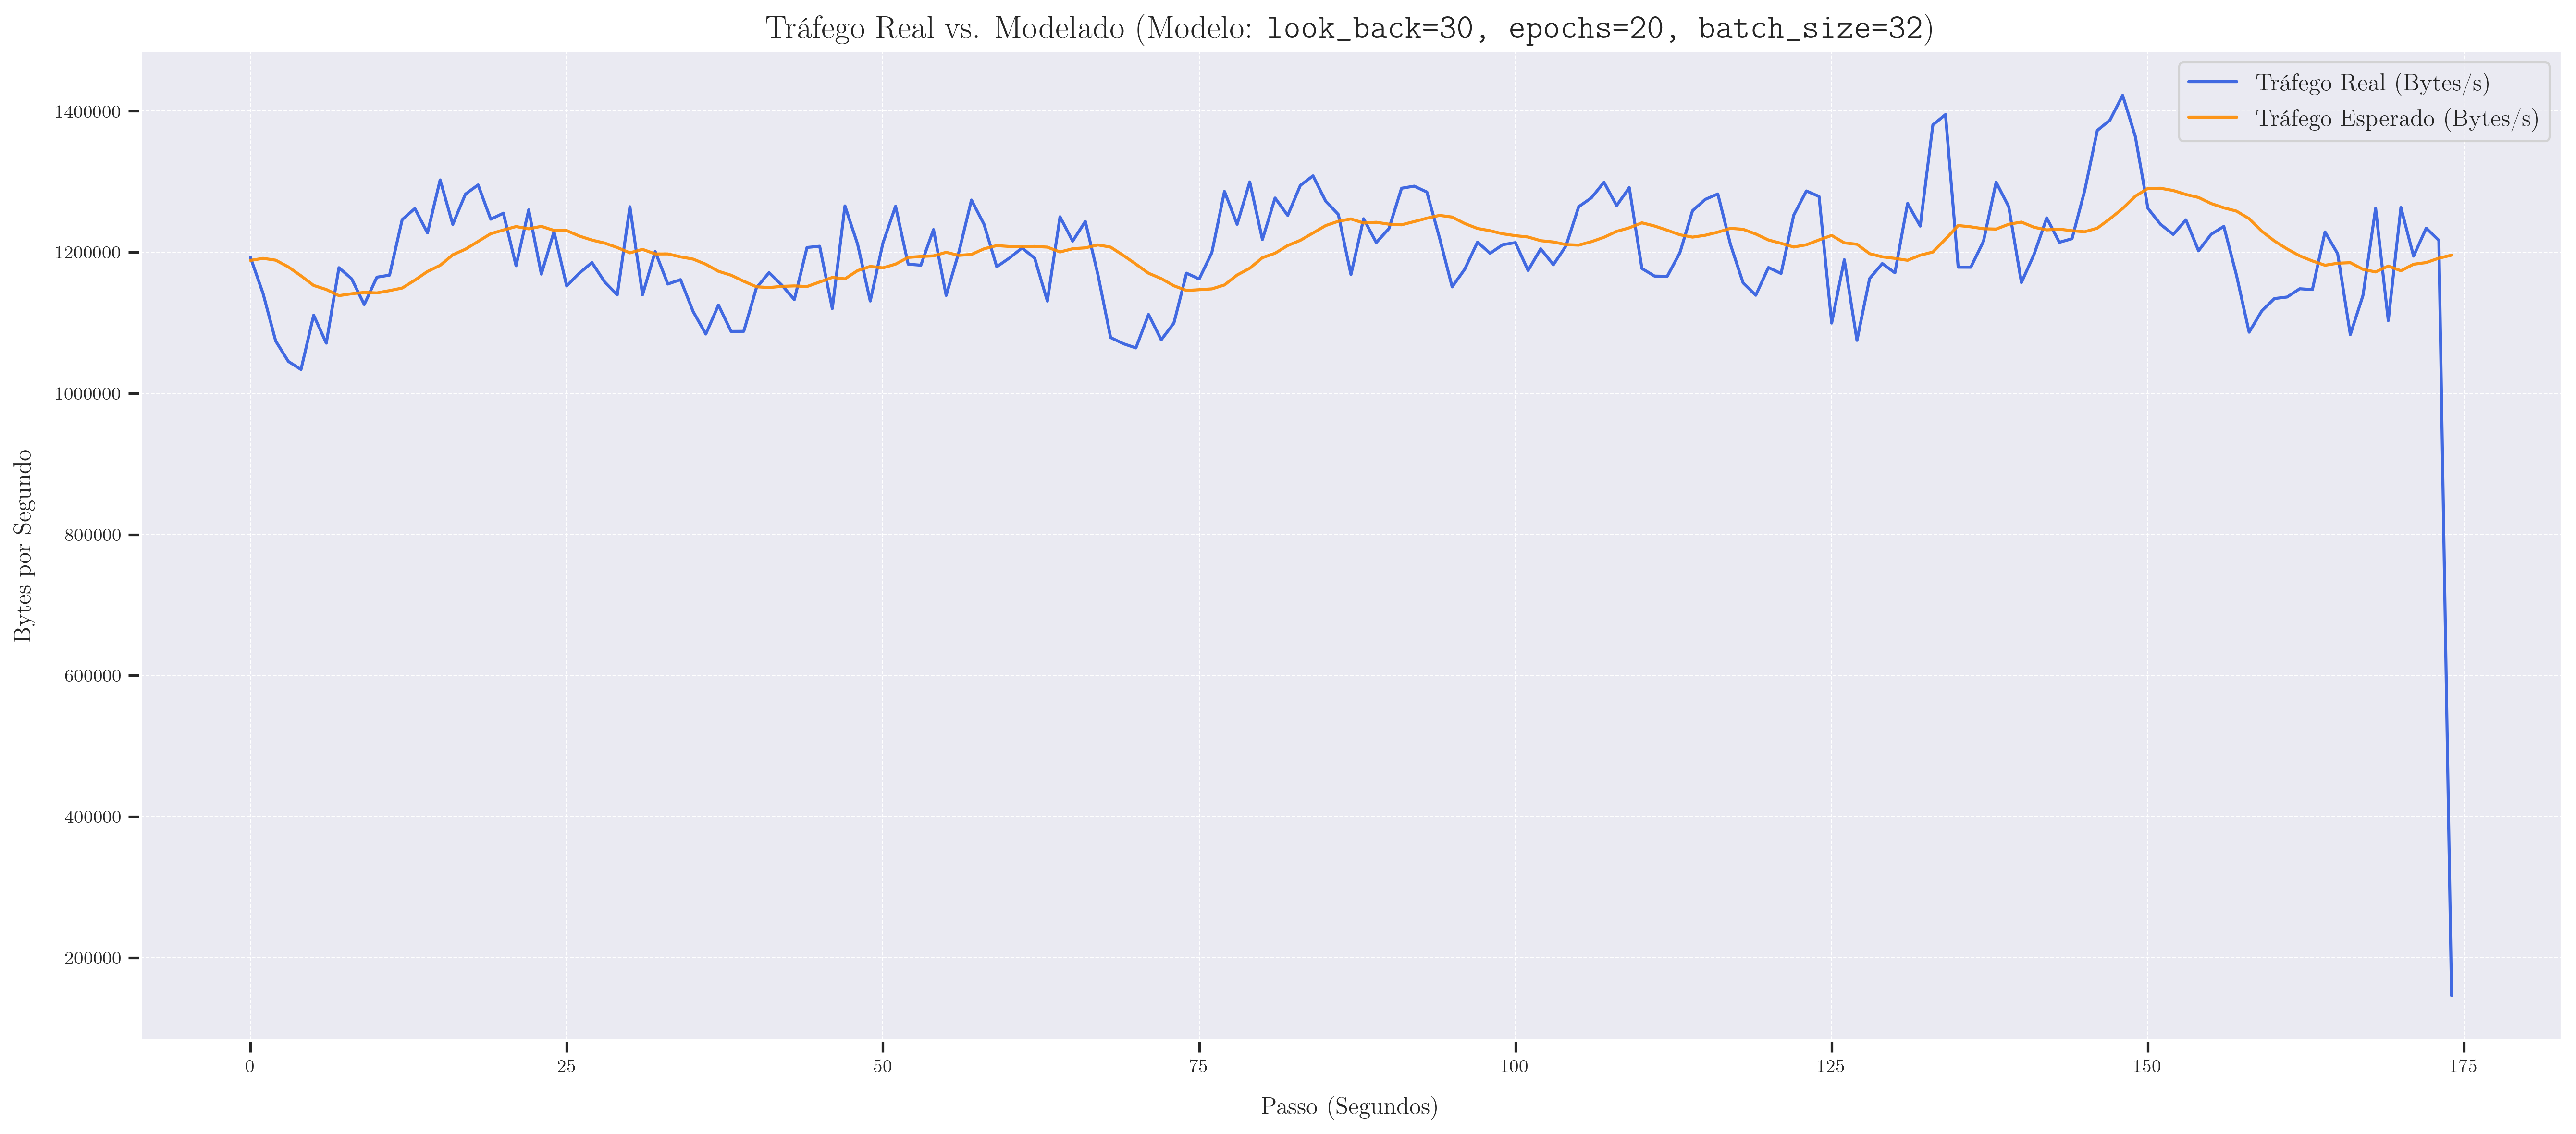
\includegraphics[width=0.95\textwidth]{resource/200701251400.prediction.e20.b32.png}
    \caption{Previsão do modelo com \emph{batch size} de 32 no \emph{dataset} curto.}
    \label{fig:modeling-prediction-reduced}
\end{figure}

Conforme observado na \Cref{tab:modeling-mse-reduced} e na \Cref{fig:modeling-prediction-reduced}, a redução
dos hiperparâmetros de treinamento não resultou em uma diferença significativa na performance ou no
comportamento do modelo em comparação com a execução principal. Isso reforça a conclusão de que a performance
do modelo, neste caso, é mais limitada pela sua arquitetura simples do que pela otimização fina dos
hiperparâmetros de treinamento.

\clearpage
\section{Discussão Crítica}

A análise dos resultados revela um comportamento dual do modelo LSTM, que varia drasticamente com a natureza
do \emph{dataset} utilizado.

No \emph{dataset} de 15 minutos, que exibe um tráfego relativamente estável, o modelo foi capaz de aprender a
tendência geral e a sazonalidade de 60 segundos identificada na EDA. A previsão, embora mais suave que os
dados reais, seguiu a trajetória da série. Isso demonstra a capacidade da arquitetura LSTM de capturar
padrões de curto e médio prazo quando o comportamento da rede não apresenta variações extremas.

Em contraste, no \emph{dataset} de 9 horas, o desempenho do modelo foi paradoxal. Por um lado, ele se tornou
um preditor extremamente preciso da linha de base do tráfego. Os valores de MSE foram ordens de magnitude
menores, pois o modelo aprendeu a prever com exatidão os longos períodos de baixa atividade. Por outro lado,
ele falhou completamente em antecipar os \emph{bursts} de tráfego súbitos e de alta magnitude. O modelo
tratou esses picos como ruído imprevisível, mantendo sua previsão próxima da média histórica e não
conseguindo se adaptar a esses eventos de "cisne negro".

Essa limitação é uma consequência direta da simplicidade da arquitetura do modelo. Uma única camada LSTM,
embora eficaz para padrões regulares, não possui a capacidade de modelar a natureza inerentemente "ruidosa" e
multifacetada do tráfego de internet, que é influenciado por uma infinidade de fatores, como o controle de
congestionamento do TCP, a agregação de milhares de fluxos independentes e eventos externos imprevisíveis.

\subsection{Conclusão}

Em síntese, o projeto demonstrou com sucesso a viabilidade de utilizar uma arquitetura LSTM simples para
modelar e prever o volume de tráfego de rede. A análise exploratória foi fundamental para guiar a seleção de
hiperparâmetros, como a janela de \emph{look-back}, e para interpretar o comportamento do modelo.

A principal vantagem da abordagem foi a capacidade do modelo de aprender tendências e padrões sazonais de
longo prazo, resultando em uma previsão muito precisa da linha de base do tráfego. No entanto, sua principal
limitação foi a incapacidade de prever os \emph{bursts} de curta duração, que são de grande importância para
aplicações como detecção de anomalias ou planejamento de capacidade em tempo real.

Para trabalhos futuros, a performance poderia ser aprimorada com a exploração de arquiteturas mais complexas.
Modelos com múltiplas camadas LSTM, LSTMs bidirecionais, ou a incorporação de mecanismos de atenção poderiam
capacitar o modelo a aprender relações temporais mais sofisticadas. Além disso, a engenharia de
\emph{features}, incluindo variáveis como a distribuição de protocolos por segundo ou a hora do dia como uma
entrada explícita, poderia fornecer ao modelo um contexto mais rico, melhorando sua capacidade de prever os
picos de tráfego e tornando-o uma ferramenta mais robusta e prática para o gerenciamento de redes.

\clearpage
\appendix

\section{Scripts de Coleta e Processamento}

\begin{ghostbox}
    \captionsetup{type=listing}
    \inputminted[samepage=false]{python}{../network_traffic_predictor/download.py}
    \caption{Script \texttt{download.py} para download e extração dos arquivos PCAP.}
    \label{lst:script-download}
\end{ghostbox}

\begin{ghostbox}
    \captionsetup{type=listing}
    \inputminted[samepage=false]{python}{../network_traffic_predictor/preprocess.py}
    \caption{Script \texttt{preprocess.py} para processamento paralelo do arquivo PCAP e geração do dataset
    em formato Parquet.}
    \label{lst:script-preprocess}
\end{ghostbox}

\section{Scripts de Análise e Treinamento}

\begin{ghostbox}
    \captionsetup{type=listing}
    \inputminted[samepage=false]{python}{../network_traffic_predictor/analysis.py}
    \caption{Script \texttt{analysis.py} para a Análise Exploratória dos Dados.}
    \label{lst:script-analysis}
\end{ghostbox}

\begin{ghostbox}
    \captionsetup{type=listing}
    \inputminted[samepage=false]{python}{../network_traffic_predictor/train.py}
    \caption{Script \texttt{train.py} para o treinamento e avaliação do modelo LSTM.}
    \label{lst:script-train}
\end{ghostbox}


\end{document}
